% $Header: /cvsroot/latex-beamer/latex-beamer/solutions/conference-talks/conference-ornate-20min.en.tex,v 1.6 2004/10/07 20:53:08 tantau Exp $

\documentclass{beamer}
%\documentclass[handout]{beamer}
%\usepackage{pgfpages}
%\pgfpagesuselayout{2 on 1}[a4paper,border shrink=5mm]

% This file is a solution template for:

% - Talk at a conference/colloquium.
% - Talk length is about 20min.
% - Style is ornate.



% Copyright 2004 by Till Tantau <tantau@users.sourceforge.net>.
%
% In principle, this file can be redistributed and/or modified under
% the terms of the GNU Public License, version 2.
%
% However, this file is supposed to be a template to be modified
% for your own needs. For this reason, if you use this file as a
% template and not specifically distribute it as part of a another
% package/program, I grant the extra permission to freely copy and
% modify this file as you see fit and even to delete this copyright
% notice.


\mode<presentation>
{
%  \usetheme{Warsaw}
%  \usetheme{Boadilla}
%  \usetheme{Goettingen}
%  \usetheme{Hannover}
%  \usetheme{Madrid}
%  \usetheme{Marburg}
%  \usetheme{Montpellier}
%  \usetheme{Pittsburgh}
  \usetheme{Hawke}
  % or ...

  \setbeamercovered{transparent}
  % or whatever (possibly just delete it)
}


\usepackage[english]{babel}
% or whatever

\usepackage[latin1]{inputenc}
% or whatever

\usepackage{times}
\usepackage[T1]{fontenc}
% Or whatever. Note that the encoding and the font should match. If T1
% does not look nice, try deleting the line with the fontenc.

\usepackage{multimedia}


%%%%%%
% My Commands
%%%%%%

\newcommand{\ml}{{\sc matlab}}
\newcommand{\bb}{{\boldsymbol{b}}}
\newcommand{\bx}{{\boldsymbol{x}}}
\newcommand{\by}{{\boldsymbol{y}}}
\newcommand{\bfm}[1]{{\boldsymbol{#1}}}

%%%%

\title[Lecture 14] % (optional, use only with long paper titles)
{Lecture 14 - Adaptive and Gaussian Quadrature}

% \subtitle
% {Include Only If Paper Has a Subtitle}

\author[I. Hawke] % (optional, use only with lots of authors)
{I.~Hawke}
% - Give the names in the same order as the appear in the paper.
% - Use the \inst{?} command only if the authors have different
%   affiliation.

\institute[University of Southampton] % (optional, but mostly needed)
{
%  \inst{1}%
  School of Mathematics, \\
  University of Southampton, UK
}
% - Use the \inst command only if there are several affiliations.
% - Keep it simple, no one is interested in your street address.

\date[Semester 1] % (optional, should be abbreviation of conference name)
{MATH3018/6141, Semester 1}
% - Either use conference name or its abbreviation.
% - Not really informative to the audience, more for people (including
%   yourself) who are reading the slides online

\subject{Numerical methods}
% This is only inserted into the PDF information catalog. Can be left
% out.



% If you have a file called "university-logo-filename.xxx", where xxx
% is a graphic format that can be processed by latex or pdflatex,
% resp., then you can add a logo as follows:

\pgfdeclareimage[height=0.5cm]{university-logo}{mathematics_7469}
\logo{\pgfuseimage{university-logo}}



% Delete this, if you do not want the table of contents to pop up at
% the beginning of each subsection:
%  \AtBeginSubsection[]
%  {
%    \begin{frame}<beamer>
%      \frametitle{Outline}
%      \tableofcontents[currentsection,currentsubsection]
%    \end{frame}
%  }
\AtBeginSection[]
{
  \begin{frame}<beamer>
    \frametitle{Outline}
    \tableofcontents[currentsection]
  \end{frame}
}


% If you wish to uncover everything in a step-wise fashion, uncomment
% the following command:

%\beamerdefaultoverlayspecification{<+->}


\begin{document}

\begin{frame}
  \titlepage
\end{frame}

\section{Adaptive Quadrature}

\subsection{Adaptive Quadrature}

\begin{frame}
  \frametitle{Minimizing cost}

  The aim of numerical quadrature is to compute
  \begin{equation*}
    \int_a^b f(x) \, \text{d}x
  \end{equation*}
  where $f$ is a real function of a single variable $x$.

  \vspace{1ex}

  Looked at polynomial quadrature with equally spaced nodes. Can be
  inefficient and inaccurate.  \pause

  \vspace{1ex}

  Efficiency requires minimizing the number of function evaluations,
  which means minimizing the number of nodes.  Either
  \begin{itemize}
  \item Use standard quadrature methods, placing nodes depending on
    the local behaviour of the function $f$, or \pause
  \item Use methods that give the best accuracy for a ``generic''
    function $f$.
  \end{itemize}

\end{frame}

\begin{frame}
  \frametitle{Adaptive Quadrature}

  The aim of adaptive quadrature is to compute the integral
  \begin{equation*}
    \int_a^b f(x) \, \text{d}x
  \end{equation*}
  for arbitrary $f$ to a given tolerance $\epsilon$.

  \vspace{1ex}

  Error depends on derivatives of $f$ and the spacing $h$. Most
  efficient to put more nodes (decrease $h$) where the function varies
  rapidly. \pause

  \vspace{1ex}

  Adaptive quadrature therefore
  \begin{enumerate}
  \item Computes an approximation with few subintervals;
  \item Estimates the error on each subinterval;
  \item Subdivides subintervals where error is ``too large''.
  \end{enumerate}

\end{frame}

\begin{frame}
  \frametitle{Example subdivision}

  \begin{center}
    \includegraphics<1|handout:0>[height=0.7\textheight]{figures/Adaptive0}
    \includegraphics<2|handout:0>[height=0.7\textheight]{figures/Adaptive1}
    \includegraphics<3>[height=0.7\textheight]{figures/Adaptive2}
  \end{center}
  An example of the subintervals created by adaptive quadrature.

\end{frame}

\begin{frame}
  \frametitle{Estimating the error}

  Recursively dividing an interval into two equal subintervals is
  straightforward. But how do we choose which intervals need
  subdividing? For this we need some error measure. \pause

  \vspace{1ex}

  Use Richardson extrapolation. For any (sub)interval:
  \begin{enumerate}
  \item Compute $I_{2h}$; \pause
  \item Compute $I_h$; \pause
  \item If $I \simeq I_h + C h^s$ then the \emph{computable estimate of
      the error} is
    \begin{equation*}
      E_{2 h} \equiv \frac{|I_{2h} - I_h|}{2^s - 1}.
    \end{equation*}
  \end{enumerate}

\end{frame}

\begin{frame}
  \frametitle{Total vs.\ local error}

  Computable error is the \emph{local} error for one subinterval.
  Aim: To make the \emph{total} error over the \emph{whole} interval
  less than $\epsilon$. \pause

  \vspace{1ex}

  Total error bounded by the sum of the errors in each subinterval,
  \begin{equation*}
    |{\cal E}| \leq \sum_{\text{intervals } j} |{\cal E}_j|.
  \end{equation*} \pause

  Expect ${\cal E}_j$ to be proportional to the width of the
  subinterval,
  \begin{equation*}
     |{\cal E}_j| \leq D (x_j - x_{j-1}).
  \end{equation*} \pause

  If we bound the error on each subinterval by
  \begin{equation*}
     |{\cal E}_j| \leq \frac{\epsilon}{b - a} (x_j - x_{j-1})
  \end{equation*}
  then the resulting total error ${\cal E}$ will be less than our
  required tolerance $\epsilon$.

\end{frame}


\begin{frame}
  \frametitle{Example 1}

  \begin{center}
    \includegraphics<1|handout:0>[height=0.7\textheight]{figures/AdaptiveQuad1}
    \includegraphics<2|handout:0>[height=0.7\textheight]{figures/AdaptiveQuad2}
    \includegraphics<3>[height=0.7\textheight]{figures/AdaptiveQuad3}
  \end{center}
  The nodes for adaptive quadrature of a Heaviside function - the
  accuracy is $\sim 10^{-9}$ with $\sim 50$ nodes.

\end{frame}

\begin{frame}
  \frametitle{Example 2}

  \begin{center}
    \includegraphics<1|handout:0>[height=0.7\textheight]{figures/AdaptiveQuadSin1}
    \includegraphics<2>[height=0.7\textheight]{figures/AdaptiveQuadSin2}
    \includegraphics<3|handout:0>[height=0.7\textheight]{figures/AdaptiveQuadSin3}
  \end{center}
  The nodes for adaptive quadrature of a more complex function.

\end{frame}

\section{Gaussian Quadrature}

\subsection{Gaussian Quadrature}

\begin{frame}
  \frametitle{Gaussian Quadrature}

  Algorithms used so far use nodes $\{x_j\}$ to find a formula of type
  \begin{equation*}
    \int_a^b f(x) \, \text{d}x \simeq \sum_{j=1}^n w_j f_j.
  \end{equation*}
  \begin{overlayarea}{\textwidth}{0.5\textheight}
    \only<1-|handout:1->
    {
      Location of the nodes fixed in advance. Choice of
      polynomial then fixes \emph{weights} $w_j$.
    }
    \only<2-|handout:2->
    {
      In Gaussian Quadrature instead both weights \emph{and} nodes are
      to be determined.  Use this freedom to evaluate integral ``as
      accurately as possible''.
      \vspace{1ex}

    }
    \only<3|handout:2>
    {
      We have $2n$ degrees of freedom in the above formula, so
      can perfectly represent a polynomial of order
      $2n-1$. So  fix nodes and weights by ensuring
      \begin{equation*}
        \int_a^b x^s \, \text{d}x = \sum_{j=1}^n w_j x_j^s \quad
        \forall s = 0, 1, \dots, 2 n - 1.
      \end{equation*}
    }
    \only<4|handout:3>
    {
      If $f$ behaves in known ways (i.e., decays exponentially), can
      improve accuracy by introducing a \emph{weight function} $W(x)$:
      \begin{equation*}
        \int_a^b W(x) x^s \, \text{d}x = \sum_{j=1}^n w_j x_j^s
        \quad \forall s = 0, 1, \dots, 2 n - 1.
      \end{equation*}
    }
  \end{overlayarea}

\end{frame}

\begin{frame}
  \frametitle{Example}

  Gauss-Legendre quadrature on $[-1,1]$, $n=2$ nodes:
  \begin{equation*}
    \int_{-1}^1 x^s \, \text{d}x = \sum_{j=1}^n w_j x_j^s \quad
     s = 0, 1, 2, 3.
  \end{equation*} \pause

  This gives the four equations
  \begin{align*}
  &&s & = 0 : & w_1 + w_2 & = 2 &&\\
  &&s & = 1 : & w_1 x_1 + w_2 x_2 & = 0 &&\\
  &&s & = 2 : & w_1 x_1^2 + w_2 x_2^2 & = 2 / 3 &&\\
  &&s & = 3 : & w_1 x_1^3 + w_2 x_2^3 & = 0.&&
  \end{align*}
  The solution is $w_1 = 1 = w_2$, $x_1 = - 1 / \sqrt{3} = -
  x_2$. \pause

  \vspace{1ex}

  Therefore the Gauss-Legendre formula is
  \begin{equation*}
    \int_{-1}^{1} f(x) \, \text{d}x \simeq f(-1 / \sqrt{3}) +  f(1 /
    \sqrt{3}).
  \end{equation*}

\end{frame}

\begin{frame}
  \frametitle{Example: 2}

  If we allow ourself $n=3$ nodes we have to solve
  \begin{equation*}
    \int_{-1}^1 x^s \, \text{d}x = \sum_{j=1}^n w_j x_j^s \quad
     s = 0, 1, 2, 3, 4, 5.
  \end{equation*} \pause

  This has solution for the weights $w_1 = \tfrac{5}{9} = w_3$, $w_2 =
  \tfrac{8}{9}$ when evaluated at the nodes $x_1 = -
  \sqrt{\tfrac{3}{5}} = - x_3$, $x_2 = 0$. \pause

  \vspace{1ex}

  Therefore the Gauss-Legendre formula is
  \begin{equation*}
    \int_{-1}^{1} f(x) \, \text{d}x \simeq \frac{1}{9} \left( 5
      f(-\sqrt{\tfrac{3}{5}}) + 8 f(0) + 5 f(\sqrt{\tfrac{3}{5}}) \right).
  \end{equation*} \pause

  \vspace{1ex}

  In general, nodes are given by zeros of orthogonal polynomials (type
  depends on weight function).

\end{frame}


\begin{frame}
  \frametitle{Example: 2}

  If we apply the Gauss-Legendre formula with 2 nodes to
  \begin{equation*}
    \int_{-1}^{1} \cos^2 \left(\tfrac{\pi x}{2}\right) \, \text{d}x
  \end{equation*}
  then we find
  \begin{equation*}
    \int_{-1}^{1} \cos^2 \left(\tfrac{\pi x}{2}\right) \, \text{d}x
    \simeq 0.75938.
  \end{equation*} \pause


  The Gauss-Legendre formula with 3 nodes gives
  \begin{equation*}
    \int_{-1}^{1} \cos^2 \left(\tfrac{\pi x}{2}\right) \, \text{d}x
    \simeq 1.133565.
  \end{equation*} \pause

  Compare with the trapezoidal rule ($0$!) and Simpson's rule ($4/3$)
  -- the exact answer is $1$ and only two (three) function evaluations
  are needed.

\end{frame}

\begin{frame}
  \frametitle{Example: 3}

  \begin{overlayarea}{\textwidth}{0.6\textheight}
    \only<1|handout:1>
    {
      \begin{center}
        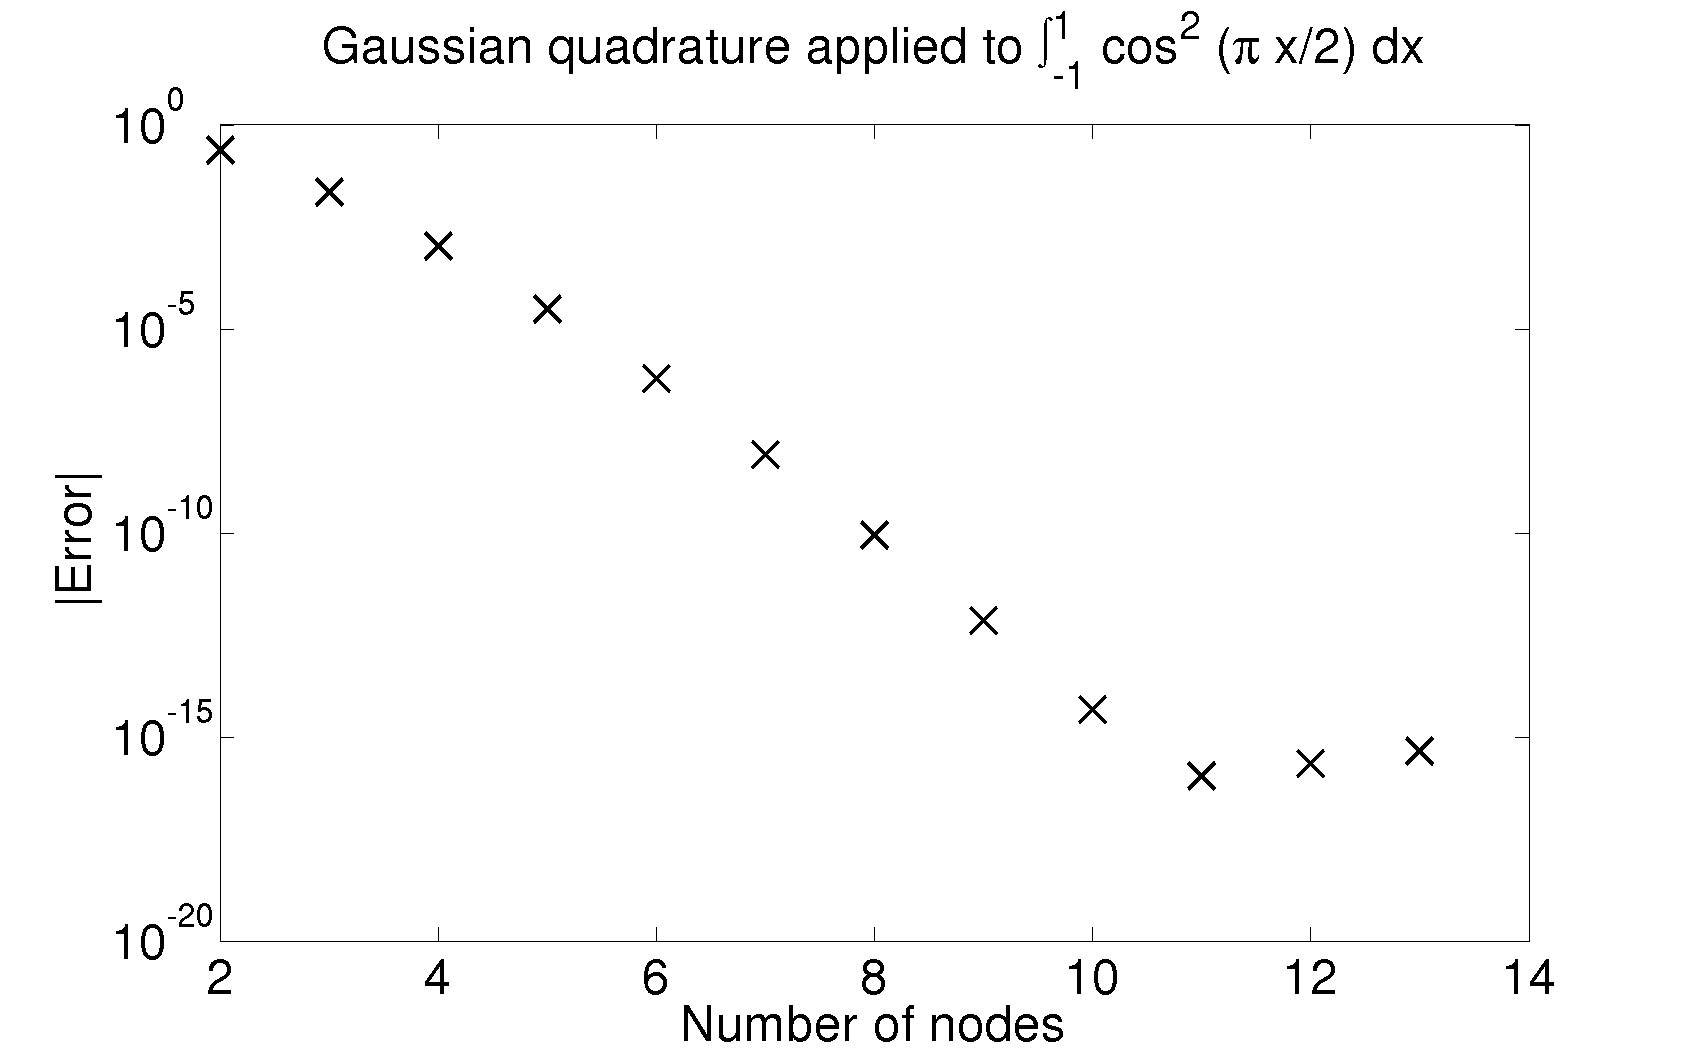
\includegraphics[height=0.6\textheight]{figures/Gauss1}
      \end{center}
    }
    \only<2|handout:2>
    {
      \begin{center}
        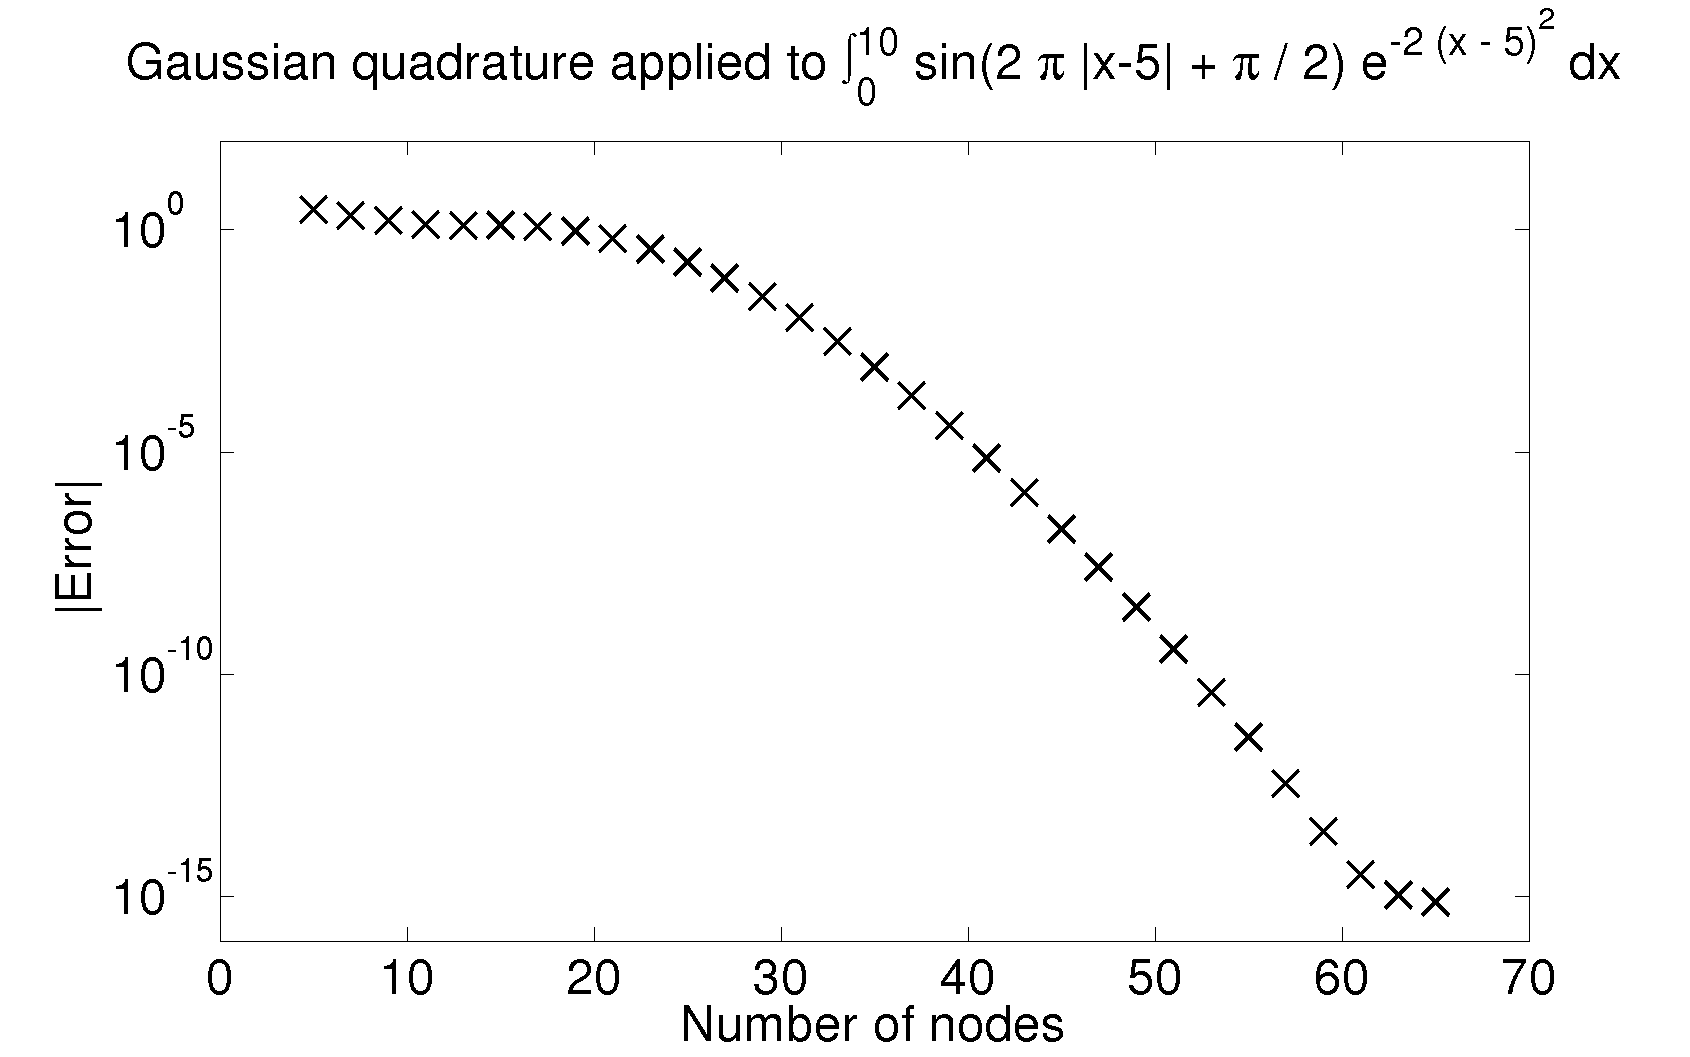
\includegraphics[height=0.6\textheight]{figures/Gauss2}
      \end{center}
    }
  \end{overlayarea}
  Simple example: very few nodes sufficient for high accuracy. \pause
  More complex example: more nodes required, but Gauss quadrature
  still more accurate than standard Newton-Cotes methods.
\end{frame}

\section{Summary}

\subsection{Summary}

\begin{frame}
  \frametitle{Summary}

  \begin{itemize}
  \item If the function is expensive to compute then to improve speed
    we need to minimize the number of nodes used.
  \item Adaptive quadrature uses standard quadrature methods
    (Simpson's rule, trapezoidal rule) by splitting the interval into
    subintervals depending on the function itself.
  \item Adaptive quadrature allows you to bound the error
    (approximately).
  \item Gaussian quadrature gives the ``best'' result for a generic
    function with a given number of nodes.
  \item The location of the nodes is computed, not given.
  \end{itemize}

\end{frame}

\end{document}



%%% Local Variables:
%%% mode: latex
%%% TeX-master: t
%%% End:
